\documentclass{article}
\usepackage{pdfpages}

\title{Team Liza \\ Milestone 3}
\author{Sam Kim \\ Kevin Geisler \\ Michael Williamson \\ Brian Collins}
\date{1-13-12}

\begin{document}

\maketitle
\newpage

\tableofcontents

\newpage

\section{System Sequence Diagrams (SSD)}

There are many SSDs that will apply to this project -- one for each assertion. 
However, each of these will follow the exact same format. Instead, we
produced a single SSD that details the flow of a test case that a developer may
write.

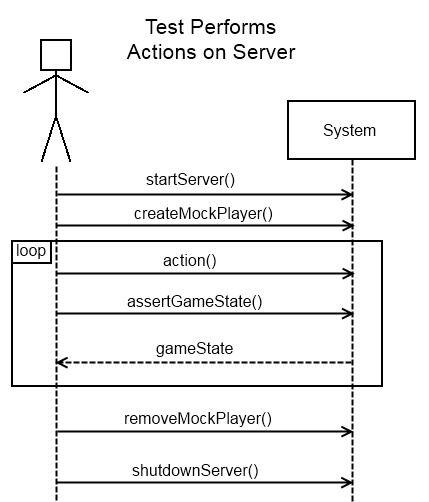
\includegraphics{ssd}

\section{Operational Contracts (OC)}

There are no operational contracts necessary for our system, as all system
calls are simple and often do not create instances of classes.

\section{Package Diagram}

There exists a degree of separation between our system and Bukkit, in the
sense that our system interacts with Bukkit, yet Bukkit is not aware of our
system. However, all of the classes in our system will all belong to the same
package, due to the high amount of interaction between classes. Because
of this, a package diagram is not applicable.

\section{Class Diagram}

The diagram is found on the following pages.
\newline

\noindent
Bukkit has two main layers: Bukkit, which is a collection of interfaces that
a plugin developer utilizes, and CraftBukkit, which is the implementation
of those interfaces. Our system will mirror this design. There is Liza, which
is a set of interfaces that inherit the Bukkit interfaces, and LizaCraft, which
is the implementation of the Liza interfaces and extends the CraftBukkit classes.
By extending the existing Bukkit and CraftBukkit, we present the API that
the developers are accustomed to, along with any new methods that may
be of use for testing, such as asserting properties. 
\newline

\noindent
There are a few new classes, however. LizaMockPlayer and its associated
implementation represent the automated player that the developer
commands. LizaMockPlayer and LizaPlayer are separated because the
latter asserts properties of any player, while the former controls only
the automated player.
\newline

\noindent
LizaListener and LizaEventExecutor handle the listening and spoofing of
events, respectively. 
\newline

\newpage
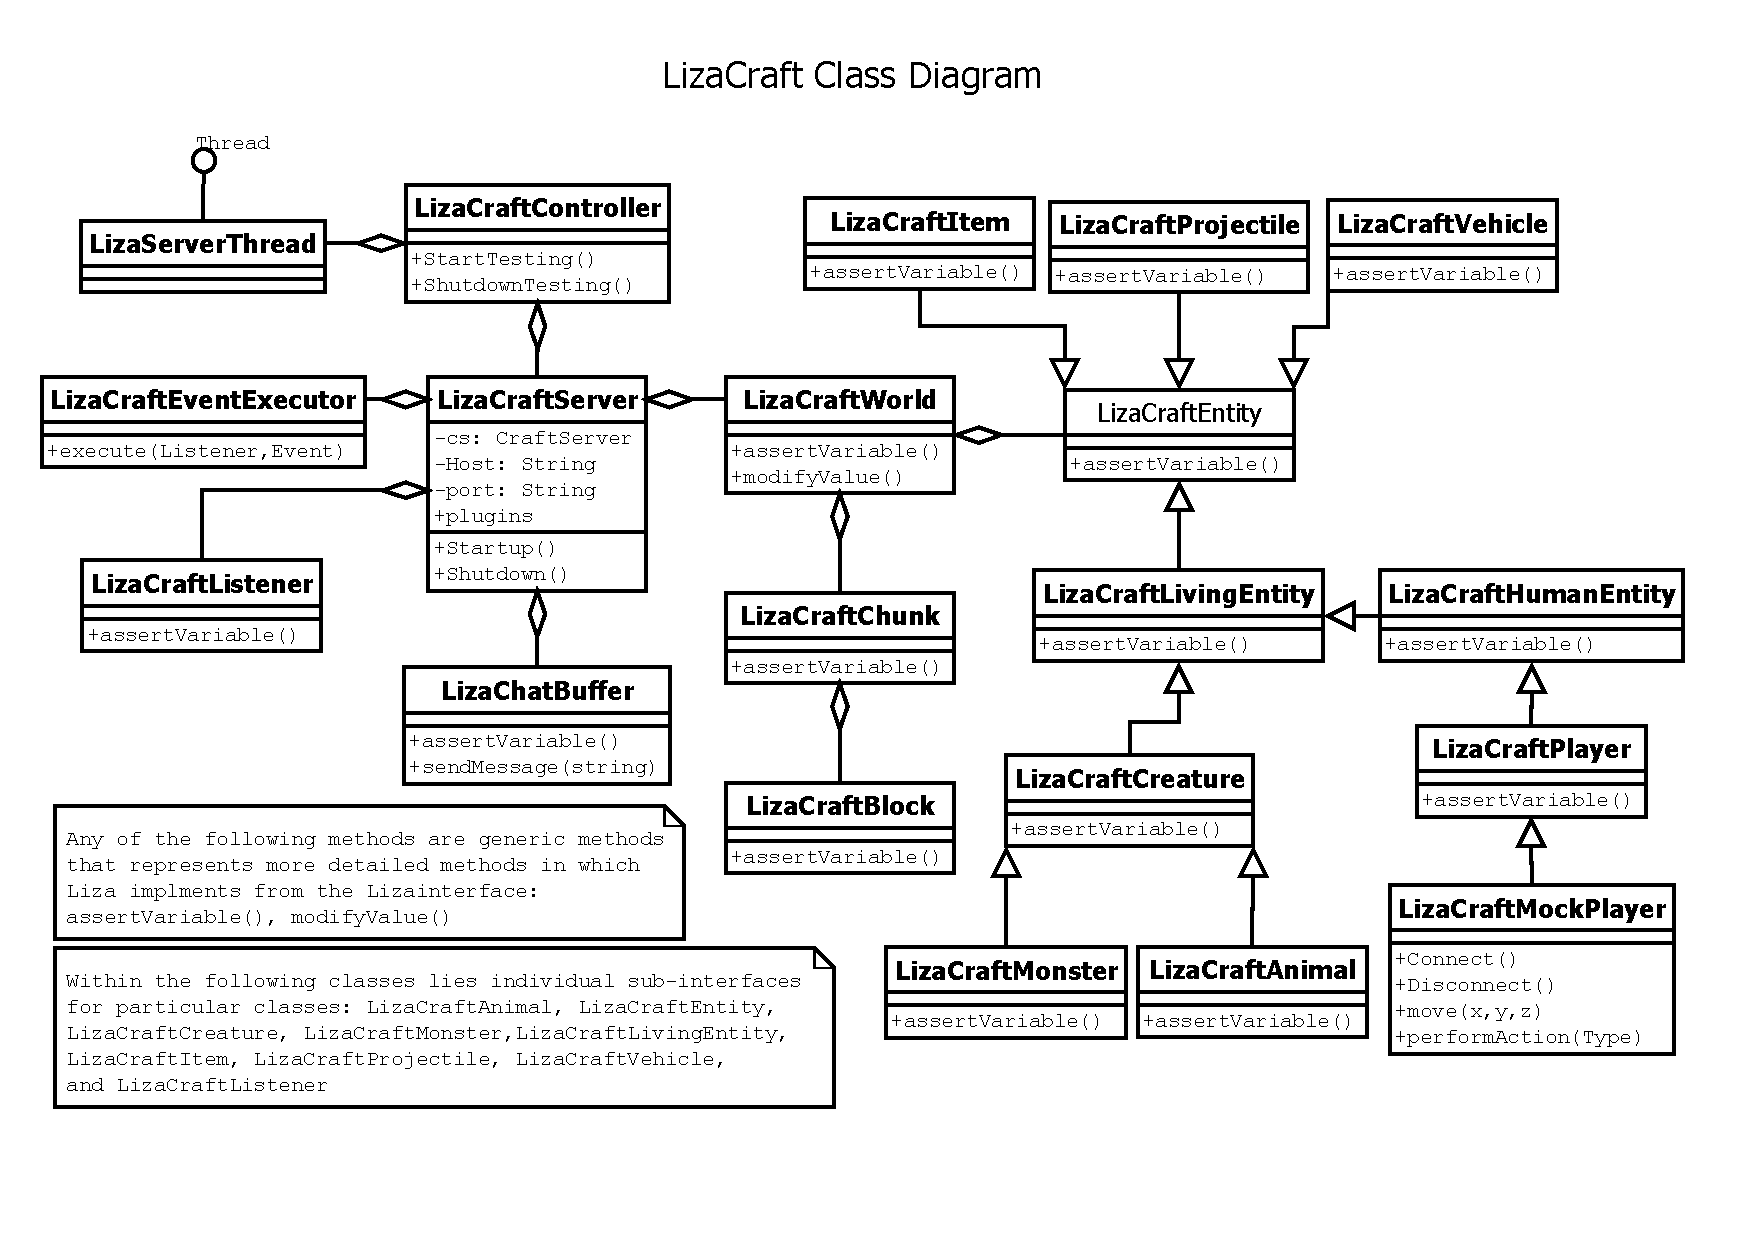
\includepdf[pages={-}]{LizaClassDiagram.pdf}

\newpage
\section{Prototype}

The prototype for this milestone is currently availble on github online at
https://github.com/geislekj/Liza

\end{document}